\chapter{Introduction}

%- Intro biology
%- beskrivelse af opgaven
%- beskrivelse af batbox
%- beskriv streaming idea
as everything is considered as stream, it becomes naturally to also do online processing on th esound stream, and take the output as video streams(waterfall spectrogram)
%- Analyse
\todo{Set the scene - publishers/subscribers, define host, nodes etc.}
\section{Users}

\begin{itemize}
	\item Biologists
	\item Developers(users, Thor)
	\item Developers(Code, John)
	\item Supervisors
	\item Backend developers
\end{itemize}

\section{Use Cases}
\myparagraph{Porpoise}
Underwater recordings are used to record Porpoise to investigate how windmills affects the Porpoise live.
\begin{itemize}
	\item {\textbf{Long recordings:}}  Hydrophones are mounted on pillars to record where the mereswines swim. The initial hypothesis was, that windmills would inhibit whales from living in that area close to windmills. However it turned out, that the whales started to breed near the windmills. Recordings are done for long periods of time.
	
	\item {\textbf{Short recordings}} During experiments, recordings of 1 min are done every 10 minute.

\end{itemize}

\myparagraph{Bats}

\todo{Insert image of batcage}
\begin{itemize}
	\item \textbf{Long recordings:} Long time recordings are used when investigating the behavior of bats in their natural habitat from ground. An example of this is when the new hospital is build in Odense. By putting up microphones the bats’ behavior can be recorded and compared to the behavior after the hospital has been build.
	
	 \item \textbf{Short recordings} Short recordings are used in Panama, as the recording boxes are not easy accessible to get near as they are mounted deep in forests. Due to lack of accessibility of the recordingsystem, the hard drives of the recordingboxes cannot easily be accessed when needed to be replaced. Therefore, they instead want to do a recording of 10 min each hour.

	\item \textbf{Trigger recordings} Trigger recordings ares used doing experiments with bats. The biologists have a bat cage, where they can conduct different experiments with bats. Sometimes it takes long before the bat does what is intended to do, so instead of doing long recordings, the biologist uses trigger recordings. When the biologist observes the bat do as intended, the biologis pushes a button, and the system saves x seconds before and after he triggered the recording. This way, he ensures that his recording contains the interesting bit, and he does not have to go through a huge amount of data, to find what he is looking for.
\end{itemize}
\todo{Figure of trigger recording}

\myparagraph{Frogs}
\begin{itemize}
	\item \textbf{Long recordings:} Frogs are recorded in their natural habitat in order to verify theoretical models of their croaking. The recordings are usually done overnight where the croaking is saved to a local disk. The bat boxes record frogs by using 8 microphones mounted in different heights and different distances. This data collected from the batboxes can be used to verify models in RANA.
\end{itemize}


\myparagraph{Skype for birds}
\todo{Insert image of setup}
\begin{itemize}
	\item \textbf{Long recordings} The idea is to tamper with communication between two Zebra Finches to understand how the tutor bird teaches the younger bird how to chirp. The batboxes are used to record the sound from one birdcage which is then played in the second birdcage. Between recording and playing, the sound can be manipulated by an AI. Recordings are played in realtime and stored for later processing. The project also concerns with tampering with two video streams(one in each direction) between the two bird cages. 
\end{itemize}
% kasser, 


\myparagraph{Drones}
The recording system is mounted on drones in order to:
\begin{itemize}
	\item \textbf{Trigger recording}Emulate the localization of a bat by emitting ultrasonic sounds. A trigger recording is started when the ultrasonic sound is emitted, such that the bounce of the emitted signal can be recording. The bounces from the signal will arrive at the batbox again within 30 ms.
	
	\item \textbf{Long recording} Point  the drone in the direction of a bat. Using multilateration, the position of the bats is estimated. GNSS will be used to synchronize the time of the batboxes. 
\end{itemize}

\myparagraph{View recordings live}
During setup of a new system, is it desired to to view the recorded data in "realtime". This would ease the setup as the microphones' position can be adjusted while watching the live processing of the data, and it would verify the system is working
Furthermore it is wanted to be able to demonstrate the system to students or other people who has interest in the functionality of the system.

\myparagraph{Calibration}
In many setups, calibration is required to know the properties of the microphones or the relative location of the microphones.
\begin{itemize}
	\item \textbf{Geometric Calibration} When the system is used to obtain the position of one or many sound sources, the microphones need to be calibration with respect to each other. By generating several sounds which are recorded by each microphone used in the setup, the position of each microphone can be estimated using multilateration. This is often needed with multiple recording boxes.
	
	\item \textbf{Frequency Calibration} Since the microphones are not linear at all frequencies, the microphones can be calibrated such that a filter can be applied to compensate for the nonlinearity.
This is done by having a speaking pointed towards a microphone, where the speakers emits sounds at known frequencies. These sounds are recorded and used to create an equalizer that can be used to compensate

\end{itemize}

\myparagraph{Data syntheses}
Either during capture or after the capturing, processing of the must be done in order to extract knowledge from the recordings.

\begin{itemize}
	\item \textbf{Data push} In some applications, the batboxes will have access to a backend’s network where data can be streamed as they are recorded. In other applications the data is saved to a local disk, which is then manually connected to the backend where data needs to be transferred to the backend.
	
	\item \textbf{Data Analysis} It should be possible to stream data to Abacus, where it can be analyzed and processed, but should also be possible to post process the data.

	\item \textbf{Data publish} When data is processed, whether it is in realtime or post-analysis, it should be presented and published in a nice way such that biologists can easily get an overview and see important features from the recorded data. Data can be exported in different formats which could for instance be to a website such that bats position can be viewed on an online map.

\end{itemize}


\myparagraph{Other sensors}
Other types of sensors should be added to the system as metadata. In some applications a GPS should be used to synchronize time, but also to know the position of the batboxes. Several parameters such as temperature, humidity etc. affects the sound measurements, so those parameters should be saved with the recordings as metadata. 

\section{Existing system}

\begin{figure}[h!]
	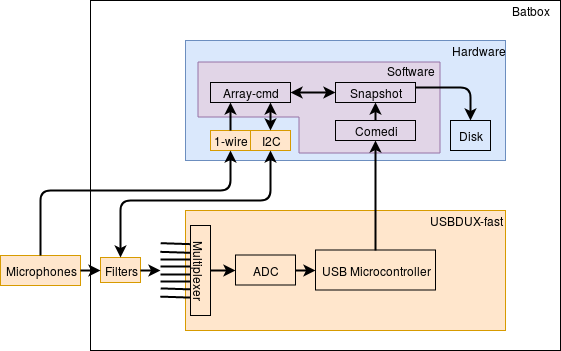
\includegraphics[width=1\textwidth]{figures/existing-system-overview.png} 
\end{figure}

\todo{Google howto export figure from draw.io to latex}

\subsection{Current setup}

As shown in section <Use-cases>, the existing system comprises of the following nodes:

snapchot is responsible for getting the auto from the usbdux/comedi module and writing the samples into files. When snapshot is initialized, it will record samples, however data is only saved to a circular buffer until it is told to write the buffer into a file. The snapshot will save part of the circular buffer to a file when it receives a “snap” command. This gives the ability to get a recording, consisting of data from a predefined time before it receives the “snap” command. Snapshot is designed to not miss out samples from the ADC.

grab has overlapping responsibility with snapshot, however: grab outputs samples to stdout and not by writing to any files. Furthermore, the implementation of the grab node is much more simple, as it has no need to maintain a circular buffering and thereby implement less memory management. If the consuming process blocks its stdin, grab will loose samples.

snapchat is responsible for communicating with snapchot and/or array-cmd depending on the application. Snapshot is run from CLI where it takes its input as parameters, and outputs by connecting to the snapshot/array-cmd.

cmd-arrays responsibilities are listed below:
Setting up the usbdux 
Handles GPIO to HMI
Saving meta-data for recordings
Determine mode of operation
Handling uuid generation
Handling recording paths
Handling connected microphones.
Being the interface to the system.
UDP + ZMQ
Hardware communication with:
LTC2637(DAC) over I2C
See flowchart of array-cmd.

trig instructs the snapshot when to do a snapshot by constructing and sending a “snap” command to either cmd-array or snapchat.

array is a script that hides the complexity of the system to ease the interface for the biologists. It is capable of initializing the system, listing connected microphones, setting options on the microphones, starting/stopping recordings etc.

Hardware - trigger line(master/slave setups)
Communication between nodes.
The interface to the recording system is either UDP or ZMQ using request/reply-pattern. Communication between the demons and CLI tools is ZMQ. Communication between threads in snapshot is also using ZMQ, however using push-patterns as ZMQ is used to do logging from busy threads.

Startup and supervision
All demons are run under supervision from the debian runit package. The runit package is both responsible for starting the nodes during startup, but also to keep the nodes running in case one of them crashes. Since runit does not provide any control of the order of startup, some fiddling has been made in order to start the snapshot and array-cmd in the proper order. From array-cmd’s run file, it tells snapshot’s supervisor, to start running.

Table of running/non-running processes.


Node name
Impl.Language
Running one-shot
Running forever
Running when used(long term)
snapshot




X


snapchat


X




grab






X
trig


X
X
X
array-cmd




X




Requirements:
Add other types of sensors (GPS, humidity, temp etc.)
Send recordings to backend when PI is online
The PI should not require internet to do recordings
Support for different hardware versions of the batbox.
Software should run on RPI
Snapshot should also be able to run on Intel in cases where powerfull enough RPI is not available.




Move files to more sensible structure
Describe different hardware versions as this makes up requirement for probing hardware

\todo{Describe and make diagrams of how to userlands tools talk through comedi modules to hardware}
\subsection{Hardware versions}
Version 1
Version 2A
Version 2B
Drone
\todo{Describe hardware. Make diagrams of the connected components}

\section{Streaming}

\subsection{Uses cases with Streaming}
\todo{Insert figures from first-handed document describing how the streaming idea applies to the different use cases}
%\myparagraph{Interface}
%As biologists are the typical user of the system, a userfriendly webinterface should be provided. Designing and implementing this is out of the scope of the report. However, it is kept in mind

